\documentclass[]{llncs} 
\usepackage{amsmath}
\usepackage{verbatim}
\usepackage{datatool}
\usepackage{tikz}
\usetikzlibrary{arrows,shapes}
\usepackage{graphics}

\newcommand{\TODO}[1]{ {\color{red}{TODO: #1} }}
\newcommand{\com}[1]{ {\color{blue}{--- #1 ---}}}

\author{Valentin Mayer-Eichberger}

\institute{NICTA \\ University of New South Wales \\
\email{valentin.mayer-eichberger@nicta.com.au}}

\title{A SAT Encoding for the AtMostSeqCard Constraint}

\begin{document} \maketitle

\section{Introduction}

Give description of the car sequencing problem and the straight
forward encoding in IP/CNF. 

The naive CNF and IP encoding of the car sequencing benchmark is
far from optimal. We can do better. 

\section{Motivation}

We are seeking an encoding that enforces GAC on the recently proposed
AtMostSeqCard constraint. This constraint is not as expressive as the
Sequence constraint but is more suited for some benchmark problems and
has a linear filtering algorithm. Here we will show that there is a
compact CNF encodings that shows good results in the benchmark set of
the CSPLIB. Furthermore we will try to improve the bounds on the set of
hard instance. 

\section{Encoding of one AtMostSeqCard}

\subsection{Encoding of counters}

\begin{figure}
\centering
\caption{A simple counter for option or class $i$ that counts to two over a sequence of 10
    sorted elements. The variables for $U$ are
set to false and the variables $L$ are set to true. The rest proper
variables of the problem $y_{i,j,k}$.}
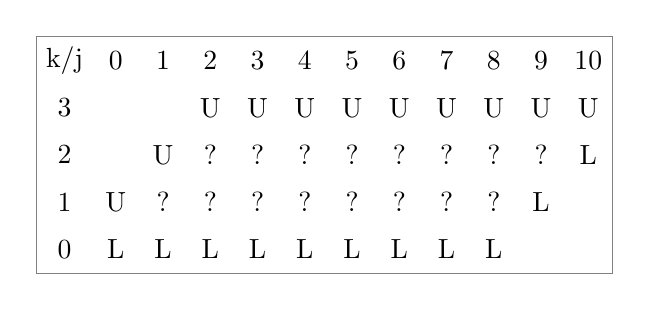
\begin{tikzpicture}
\node [matrix,ampersand replacement=\&,nodes={minimum size=6mm}]
%,nodes={fill=blue!20,minimum size=5mm}] 
    {
        \node (x) {k/j}; \& \node {0}; \& \node {1}; \& \node {2}; \& \node {3}; \& \node {4}; \& \node {5}; \& \node {6}; \& \node {7}; \& \node {8}; \& \node {9}; \& \node {10}; \\
        \node {3}; \& \node { }; \& \node { }; \& \node {U}; \& \node {U}; \& \node {U}; \& \node {U}; \& \node {U}; \& \node {U}; \& \node {U}; \& \node {U}; \& \node {U}; \\
        \node {2}; \& \node { }; \& \node {U}; \& \node {?}; \& \node {?}; \& \node {?}; \& \node {?}; \& \node {?}; \& \node {?}; \& \node {?}; \& \node {?}; \& \node {L}; \\
        \node {1}; \& \node {U}; \& \node {?}; \& \node {?}; \& \node {?}; \& \node {?}; \& \node {?}; \& \node {?}; \& \node {?}; \& \node {?}; \& \node {L}; \& \node { }; \\
        \node {0}; \& \node {L}; \& \node {L}; \& \node {L}; \& \node {L}; \& \node {L}; \& \node {L}; \& \node {L}; \& \node {L}; \& \node {L}; \& \node { }; \& \node (y) { }; \\
};
\draw[gray] (x.north west) rectangle (y.south east);
\end{tikzpicture}
\end{figure}


\subsection{Extending to AtMostSeqCard}

\section{Encoding of Carsequencing}

We need to relate the cars and options as in the problem specification.
This can be done in two ways. First the straight forward way. 

\subsection{Relating Cars and Option directly}

Let $c \in C$ be the index identifying a class and $o\in O $ be the
index for options. The problem instance gives us a mapping $m :
C\rightarrow 2^O$, relating to each class a set of options. 

\begin{equation}
    \bigwedge_{p\in P} \bigwedge_{\substack{c \in C \\ o \in m(c)}}
    \neg x_{c,p} \vee x_{o,p}
\end{equation}

and the reverse

\begin{equation}
    \bigwedge_{p\in P} (\neg x_{o,p} \vee \bigvee_{\substack{c \in C \\
    o \in m(c)}} x_{c,p})
\end{equation}

Notive in an ASP encoding this would be modelled by one rule and the
completion semantics is equivalent to this encoding. 

\subsection{The Purist's Way}

Here we will show that there is an encoding of the car sequencing
problem that does not use at all the variables $x_{i,j}$. The encoding
builds entirely on the auxiliary variables and can consistently identify
all solutions to this problem. This is rather surprising. Here the idea: 

\section{Evaluation}

Best of results that can be robustly (standard heuristics) archived by
current sat solvers. I compared newest version of minisat, lingeling,
cryptominisat, glucose and clasp and they all consistently find
solutions within 1h runtime. 

\DTLsetseparator{,}
\DTLloaddb[keys={res,set1,set2,set3,set4}]{results}{results.csv}

\begin{table}[htbp]
    \caption{}
    \centering
    \DTLdisplaydb{results}
\end{table}


This is by far better than most papers evaluating the car sequencing
problem on some specialized algorithm (e.g. branch and bound) or special
constraint (CP) or optimization (IP). 

For the set 4 a more detailed view is interesting as the benchmark
targets the optimization version of the car sequencing problem. 

\DTLsetseparator{,}
\DTLloaddb[keys={instance,ip,sat}]{set4}{set4.csv}

\begin{table}[htbp]
    \caption{Solutions to the proposed hard benchmark on the 2004 paper
    (IP) and solutions on the decision version on the SAT encoding
(SAT). }
    \centering
    \DTLdisplaydb{set4}
\end{table}


We see that already just treating the simple decision problem we can
improve the bounds given in the 2004 paper: 


\section{Extensions}

\begin{itemize}
    \item Optimizations: there are two definitions of the cost function
        for the car sequencing problem. First is to allow arbirary cars
        without any options and minimize the number of cars with
        options. And second is to minimize the number of windows that
        exceed the capacity constraint on their options. It would be
        interesting to compare both definition and to evaluate against
        published results in the literature. There are still gaps
        between known upper and lower bounds. 
    \item There is a natural extension of the AtMostSeqCard constraint
        that to a cyclic version and in the same and natural way we can
        extend the encoding given above. It would be interesting to find
        good benchmarks. 
    \item The Sequence constraint consists of a sequence of among
        constraints and we should compare this encoding to the known CNF
        encodings and filtering algorithmsin the literature. 
\end{itemize}




\end{document}
